\documentclass{standalone}
\usepackage{tikz}
\usetikzlibrary{patterns, positioning}
\usepackage[sfdefault]{ClearSans} %% option 'sfdefault' activates Clear Sans as the default text font
\usepackage[T1]{fontenc}

\begin{document}
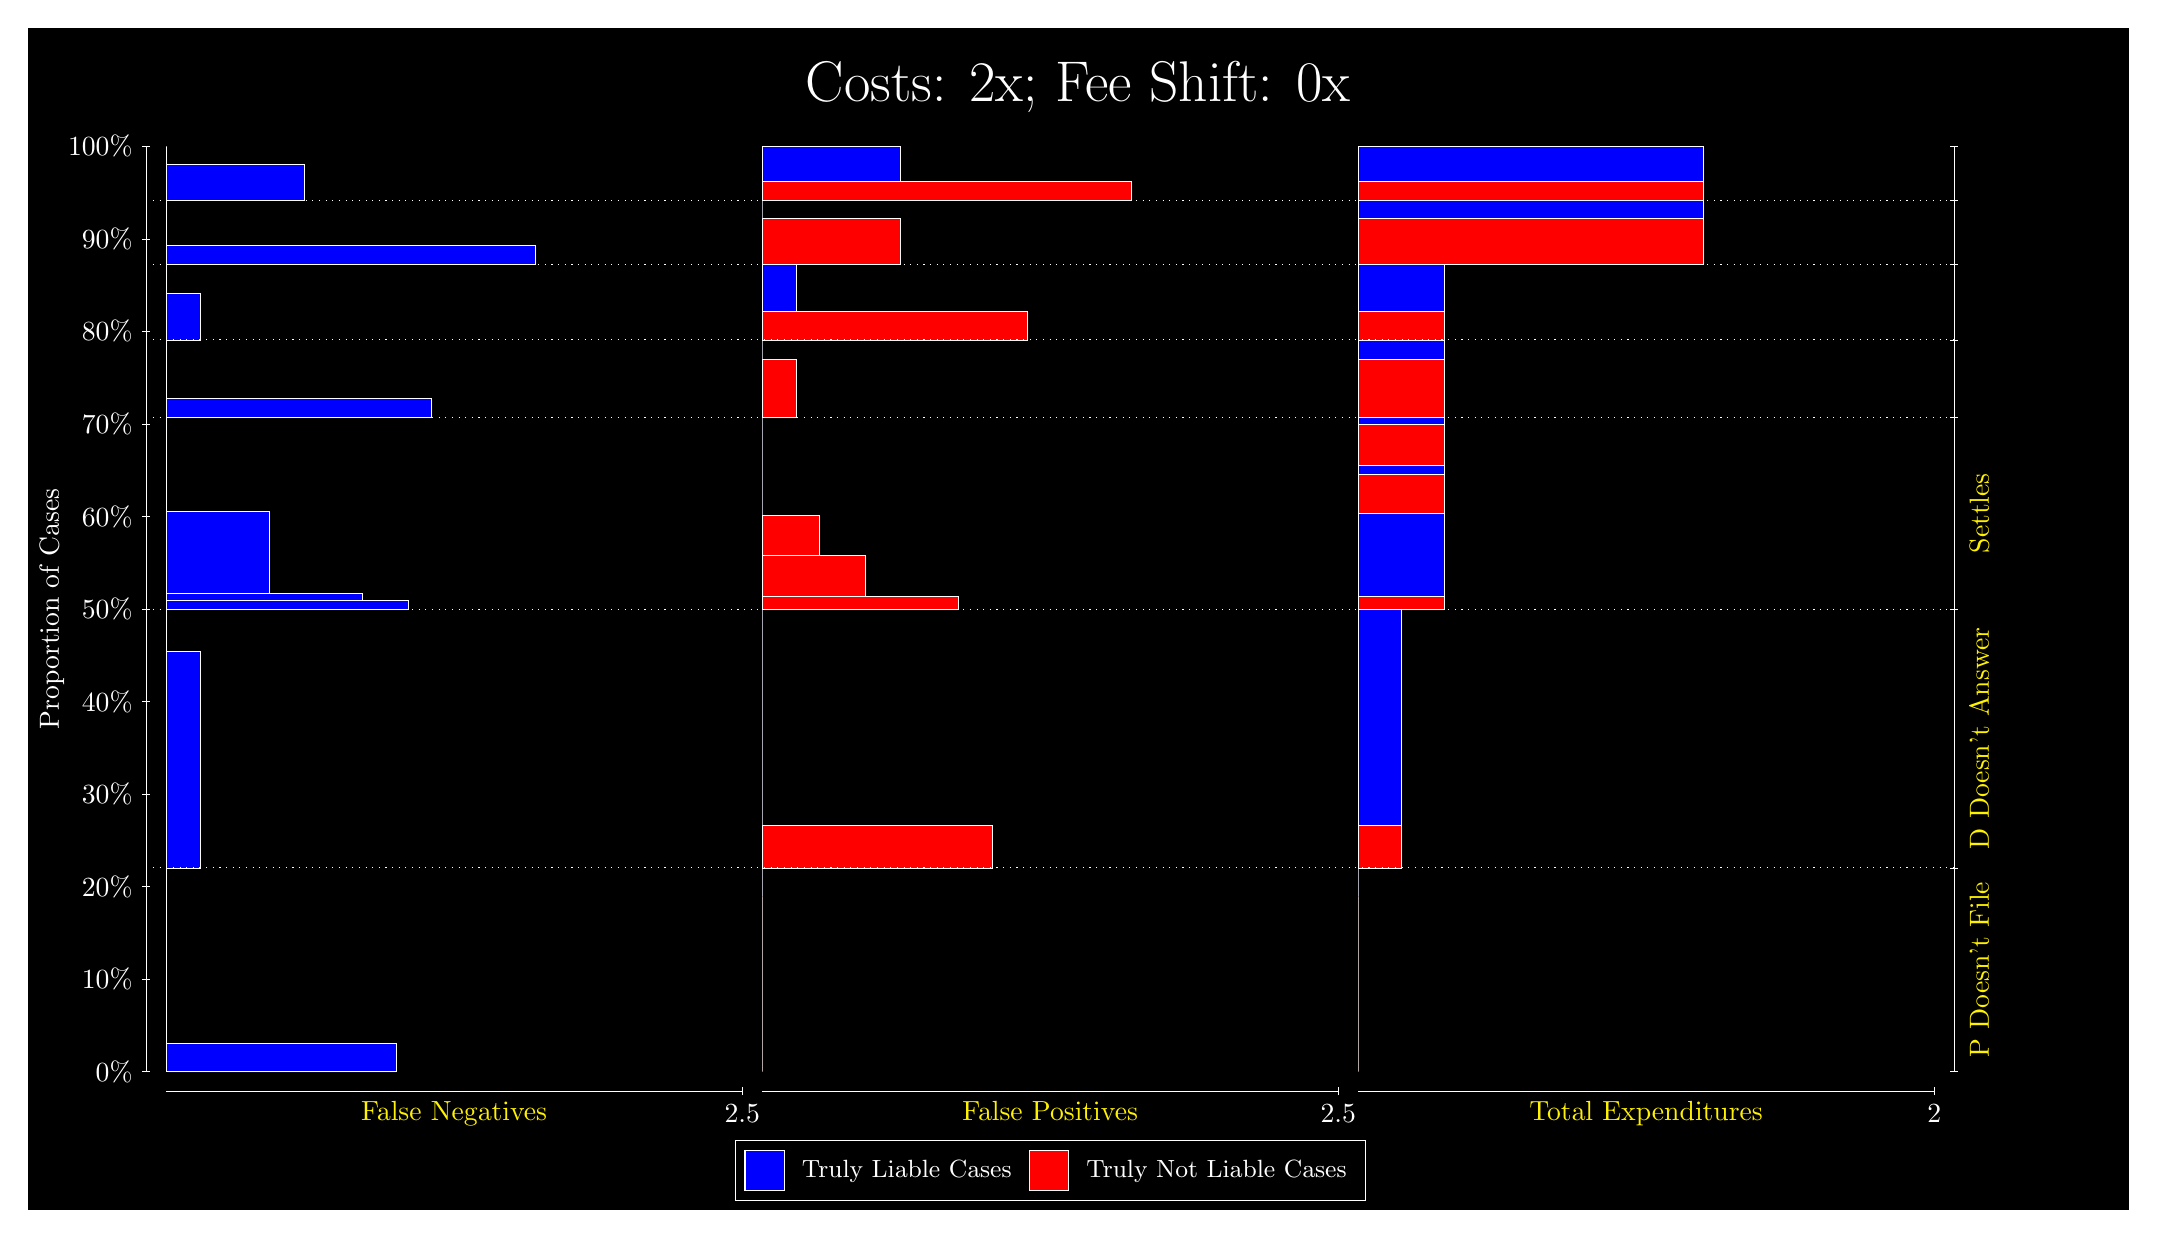
\begin{tikzpicture}
\draw[fill=black] (0,0) rectangle (26.667,15);
\draw[text=white] (0,13.5) rectangle (26.667,15) node[midway] {\huge Costs: 2x; Fee Shift: 0x};
\draw[white, very thin] (1.5,1.75) -- (1.5,13.5);
\node[rotate=90, text=white, anchor=center] at (0.3, 7.625) {Proportion of Cases};
\draw[white, very thin] (1.45,1.75) -- (1.55,1.75);
\node[text=white, anchor=east] at (1.45, 1.75) {0\%};
\draw[white, very thin] (1.45,2.925) -- (1.55,2.925);
\node[text=white, anchor=east] at (1.45, 2.925) {10\%};
\draw[white, very thin] (1.45,4.1) -- (1.55,4.1);
\node[text=white, anchor=east] at (1.45, 4.1) {20\%};
\draw[white, very thin] (1.45,5.275) -- (1.55,5.275);
\node[text=white, anchor=east] at (1.45, 5.275) {30\%};
\draw[white, very thin] (1.45,6.45) -- (1.55,6.45);
\node[text=white, anchor=east] at (1.45, 6.45) {40\%};
\draw[white, very thin] (1.45,7.625) -- (1.55,7.625);
\node[text=white, anchor=east] at (1.45, 7.625) {50\%};
\draw[white, very thin] (1.45,8.8) -- (1.55,8.8);
\node[text=white, anchor=east] at (1.45, 8.8) {60\%};
\draw[white, very thin] (1.45,9.975) -- (1.55,9.975);
\node[text=white, anchor=east] at (1.45, 9.975) {70\%};
\draw[white, very thin] (1.45,11.15) -- (1.55,11.15);
\node[text=white, anchor=east] at (1.45, 11.15) {80\%};
\draw[white, very thin] (1.45,12.325) -- (1.55,12.325);
\node[text=white, anchor=east] at (1.45, 12.325) {90\%};
\draw[white, very thin] (1.45,13.5) -- (1.55,13.5);
\node[text=white, anchor=east] at (1.45, 13.5) {100\%};

\draw[white, very thin] (24.457,1.75) -- (24.457,13.5);
\draw[white, very thin] (24.407,1.75) -- (24.507,1.75);
\node[anchor=west] at (24.407, 1.75) {};
\draw[white, very thin] (24.407,4.337) -- (24.507,4.337);
\node[anchor=west] at (24.407, 4.337) {};
\draw[white, very thin] (24.407,7.6229) -- (24.507,7.6229);
\node[anchor=west] at (24.407, 7.6229) {};
\draw[white, very thin] (24.407,10.058) -- (24.507,10.058);
\node[anchor=west] at (24.407, 10.058) {};
\draw[white, very thin] (24.407,11.043) -- (24.507,11.043);
\node[anchor=west] at (24.407, 11.043) {};
\draw[white, very thin] (24.407,12.004) -- (24.507,12.004);
\node[anchor=west] at (24.407, 12.004) {};
\draw[white, very thin] (24.407,12.817) -- (24.507,12.817);
\node[anchor=west] at (24.407, 12.817) {};
\draw[white, very thin] (24.407,13.5) -- (24.507,13.5);
\node[anchor=west] at (24.407, 13.5) {};

\draw[white, very thin, fill=blue] (1.75,1.75) rectangle (4.6775,2.1117);
\draw[white, very thin, fill=red] (1.75,2.1117) rectangle (1.75,4.337);
\draw[white, very thin, fill=blue] (1.75,4.337) rectangle (2.1891,7.0857);
\draw[white, very thin, fill=red] (1.75,7.0857) rectangle (1.75,7.6229);
\draw[white, very thin, fill=blue] (1.75,7.6229) rectangle (4.8239,7.7346);
\draw[white, very thin, fill=blue] (1.75,7.7346) rectangle (4.2384,7.8182);
\draw[white, very thin, fill=blue] (1.75,7.8182) rectangle (3.0674,8.8626);
\draw[white, very thin, fill=red] (1.75,8.8626) rectangle (1.75,10.058);
\draw[white, very thin, fill=blue] (1.75,10.058) rectangle (5.1167,10.306);
\draw[white, very thin, fill=red] (1.75,10.306) rectangle (1.75,11.043);
\draw[white, very thin, fill=blue] (1.75,11.043) rectangle (2.1891,11.637);
\draw[white, very thin, fill=red] (1.75,11.637) rectangle (1.75,12.004);
\draw[white, very thin, fill=blue] (1.75,12.004) rectangle (6.4341,12.237);
\draw[white, very thin, fill=red] (1.75,12.237) rectangle (1.75,12.817);
\draw[white, very thin, fill=blue] (1.75,12.817) rectangle (3.5065,13.267);
\draw[white, very thin, fill=red] (1.75,13.267) rectangle (1.75,13.5);
\draw[white, very thin, fill=red] (9.3189,1.75) rectangle (9.3189,3.9753);
\draw[white, very thin, fill=blue] (9.3189,3.9753) rectangle (9.3189,4.337);
\draw[white, very thin, fill=red] (9.3189,4.337) rectangle (12.246,4.8743);
\draw[white, very thin, fill=blue] (9.3189,4.8743) rectangle (9.3189,7.6229);
\draw[white, very thin, fill=red] (9.3189,7.6229) rectangle (11.807,7.7902);
\draw[white, very thin, fill=red] (9.3189,7.7902) rectangle (10.636,8.3124);
\draw[white, very thin, fill=red] (9.3189,8.3124) rectangle (10.051,8.818);
\draw[white, very thin, fill=blue] (9.3189,8.818) rectangle (9.3189,10.058);
\draw[white, very thin, fill=red] (9.3189,10.058) rectangle (9.758,10.795);
\draw[white, very thin, fill=blue] (9.3189,10.795) rectangle (9.3189,11.043);
\draw[white, very thin, fill=red] (9.3189,11.043) rectangle (12.686,11.41);
\draw[white, very thin, fill=blue] (9.3189,11.41) rectangle (9.758,12.004);
\draw[white, very thin, fill=red] (9.3189,12.004) rectangle (11.075,12.584);
\draw[white, very thin, fill=blue] (9.3189,12.584) rectangle (9.3189,12.817);
\draw[white, very thin, fill=red] (9.3189,12.817) rectangle (14.003,13.05);
\draw[white, very thin, fill=blue] (9.3189,13.05) rectangle (11.075,13.5);
\draw[white, very thin, fill=red] (16.888,1.75) rectangle (16.888,3.9753);
\draw[white, very thin, fill=blue] (16.888,3.9753) rectangle (16.888,4.337);
\draw[white, very thin, fill=red] (16.888,4.337) rectangle (17.437,4.8743);
\draw[white, very thin, fill=blue] (16.888,4.8743) rectangle (17.437,7.6229);
\draw[white, very thin, fill=red] (16.888,7.6229) rectangle (17.986,7.7902);
\draw[white, very thin, fill=blue] (16.888,7.7902) rectangle (17.986,8.8346);
\draw[white, very thin, fill=red] (16.888,8.8346) rectangle (17.986,9.3402);
\draw[white, very thin, fill=blue] (16.888,9.3402) rectangle (17.986,9.4519);
\draw[white, very thin, fill=red] (16.888,9.4519) rectangle (17.986,9.9741);
\draw[white, very thin, fill=blue] (16.888,9.9741) rectangle (17.986,10.058);
\draw[white, very thin, fill=red] (16.888,10.058) rectangle (17.986,10.795);
\draw[white, very thin, fill=blue] (16.888,10.795) rectangle (17.986,11.043);
\draw[white, very thin, fill=red] (16.888,11.043) rectangle (17.986,11.41);
\draw[white, very thin, fill=blue] (16.888,11.41) rectangle (17.986,12.004);
\draw[white, very thin, fill=red] (16.888,12.004) rectangle (21.279,12.584);
\draw[white, very thin, fill=blue] (16.888,12.584) rectangle (21.279,12.817);
\draw[white, very thin, fill=red] (16.888,12.817) rectangle (21.279,13.05);
\draw[white, very thin, fill=blue] (16.888,13.05) rectangle (21.279,13.5);
\draw[white, dotted] (1.5,4.337) -- (24.457,4.337);
\draw[white, dotted] (1.5,7.6229) -- (24.457,7.6229);
\draw[white, dotted] (1.5,10.058) -- (24.457,10.058);
\draw[white, dotted] (1.5,11.043) -- (24.457,11.043);
\draw[white, dotted] (1.5,12.004) -- (24.457,12.004);
\draw[white, dotted] (1.5,12.817) -- (24.457,12.817);
\draw[white, very thin] (1.75,1.5) -- (9.0689,1.5);
\node[text=yellow, anchor=north] at (5.4094, 1.5) {False Negatives};
\draw[white, very thin] (9.0689,1.45) -- (9.0689,1.55);
\node[text=white, anchor=north] at (9.0689, 1.45) {2.5};

\draw[white, very thin] (9.3189,1.5) -- (16.638,1.5);
\node[text=yellow, anchor=north] at (12.978, 1.5) {False Positives};
\draw[white, very thin] (16.638,1.45) -- (16.638,1.55);
\node[text=white, anchor=north] at (16.638, 1.45) {2.5};

\draw[white, very thin] (16.888,1.5) -- (24.207,1.5);
\node[text=yellow, anchor=north] at (20.547, 1.5) {Total Expenditures};
\draw[white, very thin] (24.207,1.45) -- (24.207,1.55);
\node[text=white, anchor=north] at (24.207, 1.45) {2};

\node[text=yellow, centered, rotate=90] at (24.777, 3.0435) {P Doesn't File};
\node[text=yellow, centered, rotate=90] at (24.777, 5.98) {D Doesn't Answer};
\node[text=yellow, centered, rotate=90] at (24.777, 8.8403) {Settles};





\draw (12.978300999999998,1.5) node[draw=none] (baseCoordinate) {};
\begin{scope}[align=center]
        \matrix[scale=0.5, draw=white, below=0.5cm of baseCoordinate, nodes={draw}, column sep=0.1cm]{
            \node[rectangle, draw, minimum width=0.5cm, minimum height=0.5cm, fill=blue] {}; &
            \node[draw=none, font=\small, text=white] (B) {Truly Liable Cases}; &
            \node[rectangle, draw, minimum width=0.5cm, minimum height=0.5cm, fill=red] {}; &
            \node[draw=none, font=\small, text=white] (B) {Truly Not Liable Cases}; \\
            };
\end{scope}

\end{tikzpicture}
\end{document}